% verso e anverso:
\documentclass[12pt,openright,twoside,a4paper,english,french,spanish,brazil]{abntex2}	

% apenas verso: 
%\documentclass[12pt,oneside,a4paper,english,french,spanish,brazil]{abntex2}

% -------------------------------------------------------------------------------------------------
% PACOTES
% Pacotes fundamentais 

\usepackage{cmap}				% Mapear caracteres especiais no PDF
\usepackage{lmodern}			% Usa a fonte Latin Modern
\usepackage[T1]{fontenc}		% Selecao de codigos de fonte.
\usepackage[utf8]{inputenc}		% Codificacao do documento (conversão automática dos acentos)
\usepackage{indentfirst}		% Indenta o primeiro parágrafo de cada seção.
\usepackage{color}				% Controle das cores
\usepackage{graphicx}			% Inclusão de gráficos
\usepackage{lscape}
\graphicspath{{imagens/}}
% -------------------------------------------------------------------------------------------------

% Pacotes adicionais, usados no anexo do modelo de folha de identificação
\usepackage{multicol}
\usepackage{multirow}
% -------------------------------------------------------------------------------------------------
	
% Pacotes adicionais, usados apenas no âmbito do Modelo Canônico do abnteX2
\usepackage{lipsum}				% para geração de dummy text
% -------------------------------------------------------------------------------------------------

% Pacotes de citações
\usepackage[brazilian,hyperpageref]{backref}	 % Paginas com as citações na bibl
\usepackage[alf]{abntex2cite}	% Citações padrão ABNT
% -------------------------------------------------------------------------------------------------

% CONFIGURAÇÕES DE PACOTES
% Configurações do pacote backref
% Usado sem a opção hyperpageref de backref
\renewcommand{\backrefpagesname}{Citado na(s) página(s):~}
% Texto padrão antes do número das páginas
\renewcommand{\backref}{}
% Define os textos da citação
\renewcommand*{\backrefalt}[4]{
	\ifcase #1 %
		Nenhuma citação no texto.%
	\or
		Citado na página #2.%
	\else
		Citado #1 vezes nas páginas #2.%
	\fi}%
% -------------------------------------------------------------------------------------------------


% Informações de dados para CAPA e FOLHA DE ROSTO
\titulo{ESTUDO DE DESENVOLVIMENTO HÍBRIDO PARA UM SISTEMA DE CONTROLE DE VENDAS PET SHOP}
\autor{Wesley Gomes da Silva}
\local{Palmas - TO}
\data{2013}
\instituicao{%
  Faculdade Católica do Tocantins
  \par
  Curso Sistemas de Informação
  }
\tipotrabalho{Relatório Final de Estágio}
% O preambulo deve conter o tipo do trabalho, o objetivo, 
% o nome da instituição e a área de concentração 
\preambulo{Projeto apresentado como requisito parcial para aprovação na disciplina de Estágio Supervisionado I do Curso de Sistemas de Informação, da Faculdade Católica do Tocantins (FACTO), sob a orientação do professor MsC. Marco Antônio Firmino de Sousa.}
% -------------------------------------------------------------------------------------------------


% Configurações de aparência do PDF final

% alterando o aspecto da cor azul
\definecolor{blue}{RGB}{41,5,195}

% informações do PDF
\makeatletter
\hypersetup{
     	%pagebackref=true,
		pdftitle={\@title}, 
		pdfauthor={\@author},
    	pdfsubject={\imprimirpreambulo},
	    pdfcreator={LaTeX with abnTeX2},
		pdfkeywords={abnt}{latex}{abntex}{abntex2}{relatório técnico}, 
		colorlinks=true,       		% false: boxed links; true: colored links
    	linkcolor=blue,          	% color of internal links
    	citecolor=blue,        		% color of links to bibliography
    	filecolor=magenta,      		% color of file links
		urlcolor=blue,
		bookmarksdepth=4
}
\makeatother
% -------------------------------------------------------------------------------------------------

% Espaçamentos entre linhas e parágrafos 
% O tamanho do parágrafo é dado por:
\setlength{\parindent}{1.3cm}

% Controle do espaçamento entre um parágrafo e outro:
\setlength{\parskip}{0.2cm}  % tente também \onelineskip
% -------------------------------------------------------------------------------------------------


% compila o indice
\makeindex
% -------------------------------------------------------------------------------------------------


% Início do documento
\begin{document}

% Retira espaço extra obsoleto entre as frases.
\frenchspacing 

% ----------------------------------------------------------
% ELEMENTOS PRÉ-TEXTUAIS
% ----------------------------------------------------------
% \pretextual

% ---
% Capa
% ---
\imprimircapa
% ---

% ---
% Folha de rosto
% (o * indica que haverá a ficha bibliográfica)
% ---
\imprimirfolhaderosto*
% ---

% ---
% Anverso da folha de rosto:
% -------------------------------------------------------------------------------------------------

% Agradecimentos
% ---
\begin{agradecimentos}
Agradeço em primeiro lugar a Deus o meu grande guia, por ter me abençoado com a chance de cursar em uma grande faculdade como a CATOLICA DO TOCANTINS - FACTO e ter recebido subsídios tão ricos durante essa jornada, ao professor Marco Antonio Firmino de Sousa pela orientação e motivação para realização deste trabalho, agradeço em especial a minha família por estar ao meu lado na busca por este sonho e também aos meus amigos que souberam conviver e respeitar ainda que nem sempre compartilhássemos as mesmas idéias. E por tudo, a saudade há de ficar.

\end{agradecimentos}
% -------------------------------------------------------------------------------------------------

% ---
% RESUMO
% ---
\begin{resumo}
Desenvolvimento de aplicações móvies é uma área que está em ascensão no âmbito mundial, com isso muitos serviços virão para aproveitar o conceito de mobilidade e acessibilidade. Os dispositivos móveis são os responsáveis por este crescimento, pois eles estão cada vez mais presentes na vida das pessoas. O presente trabalho descreve uma análise técnicas em 3 softwares voltado para o ramo de pet shop, onde será apresentado uma descrição de suas principais funcionalidades afim de identificar falhas que poderão ser corrigidas e melhorandas em um novo software proposto para desenvolvimento futuro e algumas tabelas de requisitos funcionais e não-funcionais de cada software.


 \vspace{\onelineskip}
    
 \noindent
 \textbf{Palavras-chaves}: Desenvolvimento híbrido. Dispositivos  móveis. Pet shop.
\end{resumo}
% -------------------------------------------------------------------------------------------------

% Inserir somente os ítens que houver conteúdo. Veja que a lista de figuras, tabelas e lista de abreviaturas estão em branco.

% inserir lista de ilustrações
\pdfbookmark[0]{\listfigurename}{lof}
\listoffigures*
\cleardoublepage
% -------------------------------------------------------------------------------------------------


% inserir lista de tabelas
\pdfbookmark[0]{\listtablename}{lot}
\listoftables*
\cleardoublepage
% -------------------------------------------------------------------------------------------------

% inserir lista de abreviaturas e siglas
%\begin{siglas}
% \item[Fig.] Area of the $i^{th}$ component
%  \item[456] Isto é um número
%  \item[123] Isto é outro número
%  \item[lauro cesar] este é o meu nome
%\end{siglas}
% -------------------------------------------------------------------------------------------------

% inserir lista de símbolos
%\begin{simbolos}
%  \item[$ \Gamma $] Letra grega Gama
%  \item[$ \Lambda $] Lambda
%  \item[$ \zeta $] Letra grega minúscula zeta
%  \item[$ \in $] Pertence
%\end{simbolos}
% -------------------------------------------------------------------------------------------------


% inserir o sumario
%\pdfbookmark[0]{\contentsname}{toc}
%\tableofcontents*
\tableofcontents 
%\cleardoublepage
% -------------------------------------------------------------------------------------------------


% ----------------------------------------------------------
% ELEMENTOS TEXTUAIS
% ----------------------------------------------------------
\textual

% ----------------------------------------------------------
% Capitulo Introdução
% ----------------------------------------------------------
\chapter*[Introdução]{Introdução}
\section*{Contexto}
\addcontentsline{toc}{chapter}{Introdução}
% seja mais profunco, pq a sociedade precisa de mobilidade? pq há tanto dispositivo móvel? Responda isso por aqui.
Nos últimos anos, com o advento dos dispositivos portáteis a nível mundial, houve um crescimento gigantesco de aplicações web mobile, principalmente no meio coorporativo, na utilização de soluções móveis para mercado cooporativo. Devido a tamanha evolução, novas plataformas de desenvolvimento e sistemas operacionais foram criados, aumentando a complexidade e muitas vezes a curva de aprendizado. Um dos maiores problemas com a disparidade entre plataformas é, a manutenção da aplicação, controle de atualizações e custeamento de equipes de desenvolvimento com conhecimentos específicos, como: Android, iOS, BlackBerry, Windows Phone, etc.
As WebApps, são aplicações projetadas para serem executadas em diversos dispositivos móveis de diferentes sistemas operacionais se tornando os nomeados Web Apps Híbridos. Ou seja, a sua interface gráfica é adaptada para dispositivos com telas menores, utilizando conceitos como o responsive (são web sites que através de técnicas de construção do HTML5 e CSS, é possível termos a versão de um site que se modifique conforme o dispositivo utilizado com excelente visualização em plataformas e resoluções diferentes). Estas aplicações podem ser acessado de qualquer computador ou dispositivo móvel por meio de um browser conectado à internet, utilizando tecnologias específicas para serem carregadas em máquinas de “baixo” processamento e normalmente com baixa velocidade de banda da rede.\\
De acordo com a Anfalpet, em 2009 o Brasil tinha pelo menos 100 mil lojas de produtos direcionados aos animais de estimação. Desse total, 40 mil eram pet shops, lojas especializadas em oferecer produtos e serviços para animais de pequeno e médio porte. \cite{Sebrae2011}.\\
Com o desenvolviemnto desse software a grande vantagens será que além ser acessada por qualquer computador também poderá acessada por dispositivos móveis aumentando assim a quantidade de dispositivos e clientes atingidos contribuindo para que a empresa possa expandir mais seus clientes e negócios.

% Não tenho foco em detalhes técnicos. Nosso curso é atividade meio e é interessante que seu trabalho seja assim. Seu objetivo não é desenvolver técnica, mas uma aplicação para uso em um contexto na sociedade. Explique isso! Detalhe técnico você tratará mais adiante.

% ----------------------------------------------------------

% Sessao Objetivo Geral
\section*{Objetivo Geral}
Este trabalho tem como objetivo realizar um estudo sistemático de conceitos relacionados ao desenvolvimento de aplicações híbridas para dispositivos móveis. Baseado nas necessidades reais de uma empresa de pet shop, que enfrenta problemas como, conciliar todas as atividades da empresa, tendo o cliente que assumi o papel de gerente e veterinário ao mesmo tempo.
Baseado em tal relato o objetivo principal desse trabalho e pesquisar como desenvolver um sistema híbrido para diversas plataformas onde possa gerenciar toda a demanda da empresa de pet shop desde um checklist de produtos feito por um vendedor externo até a finalização de um pedido seja na empresa do cliente ou em qualquer outro lugar através dos aplicativos móveis, assim otimizando o tempo de compra dos consumidores.

% -------------------------------------------------------------------------------------------------
% Sessao Objetivo Especifico
\section*{Objetivo Específico}
\begin{itemize}
\item Realizar um estudo sobre o processo de desenvolvimento de aplicações móveis, utilizando tecnologia híbrida.
\item Realizar um estudo teórico dos tipos de aplicativos móveis, suas principais características, vantagens e desvantagens.
\item Realizar uma análise técnica de três softwares do ramo, com o intuído de descobrir funcionalidades que possam agregar no software proposto.
\item Relatar como funciona uma organização deste ramo e as vantagens de um sistema de integração.
\end{itemize}
% -------------------------------------------------------------------------------------------------

%Sessao Motivação
\section*{Motivação}
Em geral obter o maior grau de conhecimento possível sobre os conceitos de desenvolvimento híbrido e futuramente está pondo em pratica todo o conhecimento adquirido neste trabalho. 
% -------------------------------------------------------------------------------------------------

%Sessao justificativa
\section*{Justificativa}
Existem, atualmente, paradigmas principais que norteiam o desenvolvimento de soluções móveis: web, nativo e híbrido. Escolher o melhor é sempre um exercício que exige atenção aos mínimos detalhes.
Baseados nesses paradigmas de desenvolvimento para aplicativos híbridos adotamos esses paradigmas, para uma empresa de pet shop, desenvolvendo uma nova interação entre diversas plataformas, onde vendedores externos e clientes terão acesso a mais informações com mais facilidade, abordando os três paradigmas de desenvolvimento, devido à utilização da linguagem JavaScript, presente em quase todos os frameworks de desenvolvimento, os resultados sempre são significativos em termos de tempo de desenvolvimento do aplicativo, padronização de código, além da praticidade do desenvolvimento.
% -------------------------------------------------------------------------------------------------

%Sessao Procedimentos Experimentais
\chapter*[Pesquisa Bibliográfica]{Pesquisa Bibliográfica}
\addcontentsline{toc}{chapter}{Pesquisa Bibliográfica}

Como base para análise utilizarei três software de gerenciamento de vendas para empresas pet shop.

\begin{itemize}
\item Tesche \& Vasconcelos empresa localizada em Poços de Caldas – MG, responsável pelo software PetSystem que trabalha com controle de vendas de produtos para clínica veterinária e pet shop.
\item NetService Consultoria em Sistemas empresa localizada em Gurupi – TO, responsável pelo software PDVtab que trabalha no controle de vendas de produtos para pet shop.
\item Pet Shop Control é um software desenvolvido pela Devsol Softwares localizada em Porto Alegre - RS, que permite administrar sua pet shop e clínica veterinária auxiliando no gerenciamento de todos os setores de sua empresa.
\end{itemize}

% análise do primeiro software petsystem
\section*{Análise Software PetSystem}
De acorodo com o \cite{TESCHE&VASCONCELOS2013}, o PetSystem é uma ferramenta desenvolvida exclusivamente para Pet Shops e clínicas veterinárias. Com diversas funcionalidades, você terá acesso a funcionalidades como: Cadastro de clientes, animais, fornecedores, controle de contas a pagar e a receber, controle bancário, agendamento de tratamentos, caixa diário, relatórios personalizados, controle de usuários. A seguir uma lista com as principais funcionalidades de cada versão e características relacionada para o entendimento mais profundo do software.

\textbf{1.	{Permissão de acesso}}\\
Após efetuar o login no sistema, será necessário inserir permissões de acesso aos funcionários como: cadastro de produtos, cadastro de ordem de serviço, cadastro de fornecedores entre outros. A vantagens nesse serviço é o controle de acesso e restrições a serviços do sistema.

\textbf{2.	{Cadastro de Vendedores}}\\
Nesta opção vamos armazenar no sistema todos os vendedores da empresa, caso não utilize ao menos um vendedor é necessário para o sistema, você pode cadastrar neste o nome do vendedor como loja (se for o caso). A vantagens nessa função de cadastro serve exatamente para controle de vendedores específicos.

\textbf{3.	{Cadastro de Categorias de Clientes}}\\
O objetivo do Cadastro de Categorias do PETSYSTEM é criar grupo de perfil para seus clientes e fornecedores. Caso não deseje trabalhar com categorias é necessário criar ao menos uma para cadastro. O objetivo dessa função e criar categorias de clientes.

\textbf{4.	{Cadastrar Cliente}}\\
O objetivo desse cadastro de cliente e armazenar os dados dos clientes como:
Animais:\\ 
Tem por objetivo de apenas demonstrar quais animais foram cadastrados para este cliente, caso desejar cadastrar um novo Animal, poderá clicar no botão F5: Animais.
Restrições:\\ 
Podemos ver as opções de bloqueio de cliente, é importante ressaltar que nestes campos ao selecionar Não significa que o cliente está sem restrições.
Financeiro:\\ 
Pode determinar um dia padrão para os vencimentos deste cliente.
Histórico:\\ 
Temos os campos, Última compra e Valor Compras AC são campos são alimentados automaticamente pelo sistema.

\textbf{5.	{Orçamento}}\\
O usuário poderá efetuar orçamentos de diversos produtos em um formulário único contendo todos os dados dos produtos e do cliente, podendo assim efetuar a impressão e/ou exportar para um diretório especifico.
Alguns campos que serão apresentando no formulário são: Código do vendedor, código do cliente, situação do orçamento, itens do orçamento, valor do item, total do orçamento, observações, desconto unitário, desconto total, entre outros.

\textbf{6.	{Romaneio de Rotas de Cargas}}\\
Romaneio de rotas consiste em criar rotas para entregas de produtos, que é dividida em duas etapas, o primeiro passo será criar as rotas do romaneio, a segunda consiste na emissão do romaneio:
Criação de Rotas:\\
Será necessário apenas que preencha as informações da rota como por exemplo o código da rota (número), descrição, o veículo e também a placa e selecionar o funcionário. Nesta janela é obrigatório o preenchimento apenas do número da rota e descrição, os dados de veículo, as observações não são obrigatórias.
Montagem do Romaneio:\\
Após a criação das rotas e feito a montagem da rota com os produtos, em uma nova janela adicionando os seguintes item: data da carga, data da saída e do retorno, número de sua venda, número da nota fiscal, para finalizar o cadastro do romaneio clique no botão incluir, para que possa ser impresso a rota de entrega do produto. A vantagem dessa operação consiste em criar e controlar entregas de produtos, gerando uma rota para os entregadores, facilitando seu trabalho.

\textbf{7.	{Centro de Custos }}\\
Através do centro de custo podemos agrupar nossos históricos. Um exemplo para isto é a necessidade de visualizar todas as despesas fixas no mês. Ao invés de verificar uma a uma nós podemos agrupar elas em um centro de custo e depois visualizar o total de todas estas despesas em um único relatório. A vantagens dessa funcionalidade está em agrupar relatórios tanto de despesas quanto de lucros.

\textbf{8.	{Centro de Custos }}\\
Na tela Agenda, fica armazenado todos os futuros atendimentos e compromissos da empresa. A vantagem está no controle dos compromisso da empresa como: Consultas, banhos, tosa entre outros.

\textbf{9.	{Clinica}}\\
Atendimento:\\
Em atendimento irá reunir as informações indicadas em todo histórico de atendimento do animal, assim como oferece o recurso para registrar o novo atendimento registrando o prontuário. A vantagem nessa opção consiste em agendar um atendimento a um determinado animal.\\
Receituário:\\
Nesta janela poderá prescrever as receitas para os animais, assim como inserir textos rápidos de recomendações anteriormente cadastradas no sistema. A vantagem está em imprimir uma receita para o animal.


Com algumas das principais funcionalidades descritas acima, observamos com detalhes o funcionamento do software PetSystem. Funcionalidades que auxiliam funcionários a trabalhar de forma correta, dando mais agilidade no processo de gerenciamento da organização.


% análise do segundo software PDVtab
\section*{Análise Software PDVtab}
De acordo com o \cite{NetServiceConsultoria2013}, PDVtab é uma ferramenta desenvolvida exclusivamente para Pet Shops e clínicas veterinárias. Com diversas funcionalidades como: Cadastro de clientes, controle de contas a pagar e a receber, controle bancário, agendamento de tratamentos, caixa diário, relatórios personalizados, controle de usuários. A seguir uma lista com as principais funcionalidades do software. \\
\textbf{1.	{Cadastro Cliente}}\\
Existem várias funções que contemplam o cadastro de cliente, como conferência de assinatura, obtenção/gravação de assinatura para conferência, foto do cliente, Google Maps para localização do cliente (a eficácia do serviço depente exclusivamente do Goolgle Maps), Controle de Visita. A vantagens nesse cadastro que além dos dados dos clientes, e possível ver a localização do cliente, e um histórico de visitas dos mesmos.\\
\textbf{2.	{Função Vendas}}\\
A função de vendas é simplificada de forma que o usuário conhece todas as funcionalidades. É através da função vendas que o usuário poderá confeccionar um orçamento, ou seja, em uma mesma tela o usuário poderá: efetuar vendas, cadastrar cliente e efetuar um orçamento. A vantagens nessa função e agilidade e rapidez no processo, com apenas uma função e possível efetuar vendas, orçamentos e cadastrar clientes.\\
\textbf{3.	{Lançamento de Nota Fiscal}}\\
A vantagens nesse processo e a importação da nota fiscal através de um arquivo XML enviado pelo fornecedor, poupando assim de ter que digitar todos os produtos no lançamento.\\

%imagem nota fiscal
\begin{figure}[htb!]
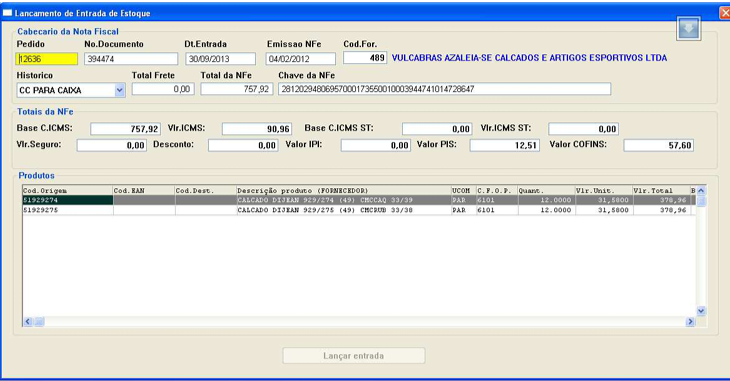
\includegraphics[scale=0.7]{nota_fiscal} 
\centering
\caption{Lançamento de entrada com a importação dos dados do XML do fornecedor} 
\cite{NetServiceConsultoriaemSistemas2013}
\label{img_nota_fiscal}
\end{figure}

\newpage
\textbf{4.	{Gráfico de Vendas e Serviços}}\\
A vantagem desse relatório utilizando gráficos do tipo pizza, e que mostra claramente o índice de lucro do total produtos e serviços vendidos durante um determinado período.

%imagem grafico de vendas e serviços
\begin{figure}[htb!]
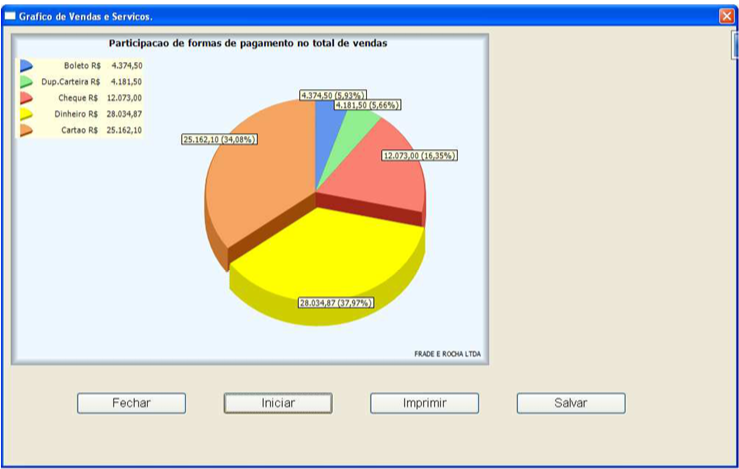
\includegraphics[scale=0.7]{grafico_vendas_servico} 
\centering
\caption{Gráfico que apresenta em forma de pizza a participação dos serviços sobre o total vendido}
\cite{NetServiceConsultoriaemSistemas2013}
\label{img_grafico_vendas_servico}
\end{figure}

%nova pagina começa aqui.
\newpage

\textbf{5.	{Gráfico de Despesas Operacionais}}\\
A grande vantagens desse tipo de relatório mostra claramente ao cliente quais os meses que houve mais despesas operacionais, assim ajudando futuramente na tomada de decisão da empresa.

%imagem grafico de despesas operacionais
\begin{figure}[htb!]
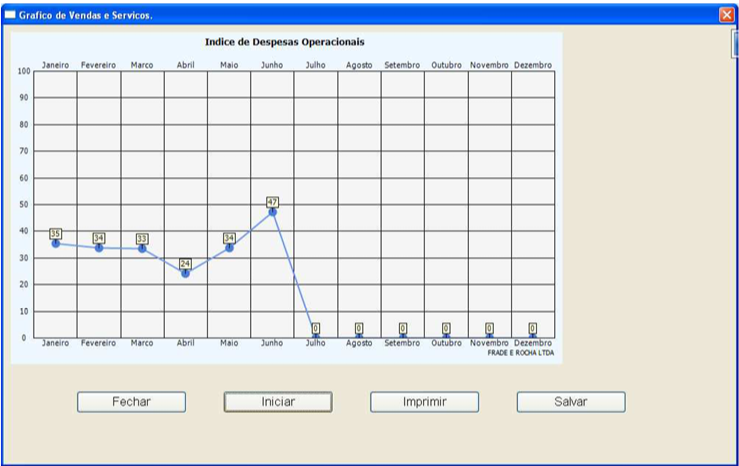
\includegraphics[scale=0.7]{grafico_despesa_operacional} 
\centering
\caption{Através desde gráfico o usuário pode acompanhar despesas operacionais}
\cite{NetServiceConsultoriaemSistemas2013}
\label{img_grafico_despesa_operacional}
\end{figure}

\newpage
\textbf{6.	{Resultado Operacional e Financeiro}}\\
A grande vantagens nesse relatório e que lista todas as despesas e lucros obtido pela empresa durante um determinado período, possibilitando assim que a tomada de decisão seja mais segura e confiante.

%imagem relatorio operacional e financeiro
\begin{figure}[htb!]
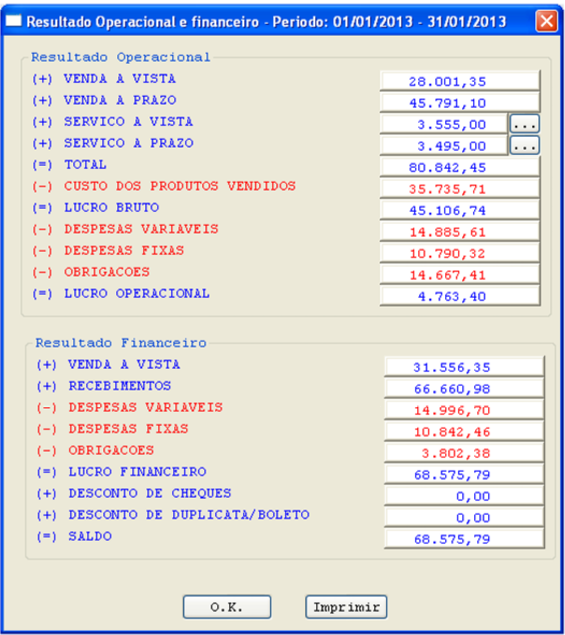
\includegraphics[scale=0.6]{relatorio_operacional_financeiro} 
\centering
\caption{Um dos principais relatórios para tomada de decisão}
\cite{NetServiceConsultoriaemSistemas2013}
\label{img_operacional_financeiro}
\end{figure}


\newpage
% análise do terceiro software Pet Shop Control
\section*{Análise Software Pet Shop Control}
De acorodo com o \cite{PetControl2013}, PetControl é um software que permite administrar sua pet shop e clínica veterinária auxiliando no gerenciamento de todos os setores de sua empresa. Através de relatórios de análises financeiras, suas decisões serão tomadas com maior segurança e precisão. Desta maneira, você conquistará uma fatia muito maior do mercado, expandindo seu negócio e aumentando seus lucros. O software pode se adaptar ao seu negócio, preservando o diferencial de mercado e seus métodos de trabalho.
A seguir uma lista com as principais funcionalidades e características relacionada para o entendimento mais profundo.

\textbf{1.	{Recuperação de Base de Dados}}\\
No caso da Pet Shop já possuir um cadastro no banco de dados, você pode restaurar os dados para preservar o histórico das informações e evitar duplicidade de cadastros.
A vantagem nessa funcionalidade e que se a empresa já tem seu banco de dados de outro sistema e decidiu mudar para esse sistema, existe a possibilidade de recuperação da base de dados assim garantindo todos os dados obtido pela empresa ao longo do tempo, minimizando problema como ter que refazer todo o cadastro de cliente por exemplo.

\textbf{2.	{Acesso ao Sistema}}\\
Após a configuração inicial do Pet Shop Control, realizada no primeiro acesso ao sistema, será necessário informar uma identificação de usuário e senha para o acesso completo ao sistema. Uma limitação encontrada e que só consegue fazer novos cadastros de usuário quem tem a senha de administrador total do sistema. A vantagem nesse tipo de restrição e exatamente privar pessoas não autorizadas a manusear o software podendo executar funções que vá a danificar ou até mesmo apagar dados de clientes ou produtos.

\textbf{3.	Pesquisar Serviços}\\
Nesta janela, no campo da busca rápida, é possível pesquisar utilizando como critério o nome do serviço, descrição, nome do grupo, código do cadastro do serviço ou utilizando o nome da categoria do serviço. A vantagem nessa funcionalidade, e listar os agendamentos de serviços efetuados.

\textbf{4.	Configurar um Serviço para Remarcar Automaticamente}\\
Essa funcionalidade habilita que um serviço, como exemplo banho em um determinado animal, possa ser remarcado automaticamente sem nenhuma interversão humana automatizando o trabalho. A vantagem nessa função e que o funcionário não precisara lembrar de um determinado serviço agendado, sendo que ele já está remarcado automaticamente, assim quando um serviço será repetido várias vezes poderá justamente se encaixar nessa função.

\textbf{5.	Pesquisa Inteligente}\\
As janelas de busca inteligente do sistema utilizam um algoritmo de última geração para filtrar os resultados de uma pesquisa. Na janela de busca dos clientes, por exemplo, é possível digitar no campo de busca rápida qualquer um dos seguintes itens para filtrar a busca: nome do proprietário, telefone, celular, e-mail, CPF, RG, código, nome do animal ou endereço. Não é necessário se preocupar com acentuação ou letras maiúsculas e minúsculas nas palavras digitadas, pois o sistema é flexível em relação a estas variações de escrita. A grande vantagem nessa função e da dinamismo e rapidez a pesquisa de um determinado cliente.

\textbf{6.	Lembretes - Quadro de Avisos}\\
O sistema dispõe de um quadro de avisos que apresenta as principais informações utilizadas no dia-a-dia da gestão de sua Pet Shop. A janela de lembretes permite visualizar um resumo das principais informações cadastradas. A vantagem desse tipo de informação e que o funcionário está à par de todos os serviços pendentes por exemplo.

\textbf{7.	Anexar Arquivos ao Cadastro de Animal}\\
Utilize esta ação para anexar exames, arquivos, fotos, vídeos e qualquer tipo de arquivo a um cadastro de animal. A vantagem nessa funcionalidade e que podemos anexar fotos dos animais, isso ajudara em uma futura venda onde os clientes poderão visualizar fotos dos animais e também exames e vídeos.

\textbf{8.	Controle de Vale Compras e Crediário dos Clientes}\\
O sistema permite que você identifique (assinale) o nível de credibilidade de seus clientes. Para isto, você pode utilizar as bandeiras existentes no cadastro do cliente. A grande vantagem e que com essa função e que saberemos exatamente aqueles clientes que mais estão comprando na loja, assim podendo ofertara-los com promoções e brindes e aqueles que possuem algum debito com a empresa, tudo atreves de bandeiras que representam os três tipos de clientes: bom relacionamento de credito, relacionamento mediano de crédito e relacionamento de crédito ruim.

\textbf{9.	Fidelidade do Cliente}\\
Você pode utilizar o sistema para criar um programa de fidelidade do cliente. Desta forma, cada compra do cliente, na loja, poderá acrescentar um valor de bônus para aquisição na loja. Uma limitação, só e capaz de efetuar essa função quem estiver com a senha do administrador. A vantagem nessa operação e que e estipulado um valor para o cliente comprar, se ele atingir esse valor, ganhar descontos em bônus automaticamente no final da compra.

\textbf{10.	Consultar Histórico de Compras de um Fornecedor}\\
Histórico de produtos comprados do fornecedor, com informações como: menor valor pago, maior valor pago e média do valor pago. A vantagem e que esse historio você saberá exatamente diferenças em valores de compras e produtos específicos anteriores.
\newpage

\textbf{11.	Enviar Mala Direta}\\
Através do envio de mala-direta aos clientes é possível divulgar sua empresa com e-mails marketing, aproximando seus clientes. Uma limitação a essa função e que tanto a empresa como o cliente deve ter um e-mail válido cadastrado no sistema antes de enviar alguma mata direta ao cliente. A principal vantagem dessa funcionalidade e a divulgação da empresa e de seus produtos aos clientes isso através do próprio sistema. Outra vantagem e que o sistema possibilita cadastrar modelos de e-mails, assim quando precisar notificar um cliente que sua conta está vencendo por exemplo, já tem um e-mail de vencimento como modelo pronto pra ser enviado.
 

Com algumas das principais funcionalidades descritas acima, observamos com detalhes o funcionamento do software Pet Shop Control. Funcionalidades que auxiliam funcionários a trabalhar de forma correta e dando mais agilidade no processo de gerenciamento da organização.
\newpage
% tabela de requisitos dos softwares
\section*{Requisitos Funcionais}
Logo abaixo uma tabela representando todos os requisitos funcionais e dos três software analisado e do software proposto para ser desenvolvido futuramente.

\newpage
\begin{landscape}
%tabela dos requisitos funcionais
\begin{table}[!htpb]
\centering
\caption{Requisitos Funcionais}\label{tab_requisitosFuncionais}
\begin{small} 
\setlength{\tabcolsep}{3pt} 
\begin{tabular}{rccccc}
    \toprule
    \multicolumn{1}{c}{\textbf{ID}} & \textbf{Descrição} & \textbf{PetSystem} & \textbf{PDVtab} & \textbf{PetControl} & \textbf{Software Proposto} \\
    \midrule
    RFC0001 & Cadastrar Animal & x & x & x & x \\
    RFC0002 & Cadastrar Proprietário & x & x & x & x \\
    RFC0003 & Buscar Animal & x & x & x & x \\
    RFC0004 & Busca Proprietário & x & x & x & x \\
    RFC0005 & Alterar Animal & x & x & x & x \\
    RFC0006 & Alterar Proprietário & x & x & x & x \\
    RFC0007 & Remover Animal & x & x & x & x \\
    RFC0008 & Remover Proprietário & x & x & x & x \\
    RFC0009 & Cadastrar Consulta & x & x & x & - \\
    RFC0010 & Cadastrar Cirurgia & x & x & x & - \\
    RFC0011 & Cadastrar Vacinação & x & x & x & - \\
    RFC0012 & Cadastrar Internação & x & x & x & - \\
    RFC0013 & Gerar Receita (da consulta) & x & x & x & - \\
    RFC0014 & Cadastrar tosa/banho & x & x & x & - \\
    RFC0015 & Registrar que vacinação já foi administrada & x & x & x & - \\
    RFC0016 & Gerar relatório (animais a serem vacinados) & x & x & x & - \\
    RFC0017 & Gerar relatório (internamento) & x & x & x & - \\
    RFC0018 & Gerar fatura Cirurgia & x & x & x & - \\
    RFC0019 & Gerar fatura Consulta & x & x & x & - \\
    RFC0020 & Gerar fatura Internamento & x & x & x & - \\
    RFC0021 & Gerar fatura tosa/Banho & x & x & x & - \\
    RFC0022 & Cadastrar Produto & x & x & x & x \\
    RFC0023 & Buscar Produto (por nome) & x & x & x & x \\
    RFC0024 & Buscar Produto (por fornecedor) & x & x & x & x \\
    RFC0025 & Registrar compra de Produto & x & x & x & x \\
    RFC0026 & Registrar venda de Produto & x & x & x & x \\
    RFC0027 & Aviso: Produto acabando & x & x & x & x \\
    RFC0028 & Gerar fatura Venda & x & x & x & x \\
    RFC0029 & Cadastrar Funcionário & x & x & x & x \\
    RFC0030 & Registrar compra de utilidades da veterinária & x & x & x & x \\
    RFC0031 & Gerar Receita & x & x & x & x \\
    RFC0032 & Pagar Cirurgia & x & x & x & - \\
    RFC0033 & Pagar Consulta & x & x & x & - \\
    \bottomrule
    \end{tabular}%
\end{small}
\end{table}
\newpage

%continuaçao tabela dos requisitos funcionais
\begin{table}[!htpb]
\centering
\caption{Continuação Requisitos Funcionais}\label{tab02_requisitosFuncionais}
\begin{small} 
\setlength{\tabcolsep}{3pt} 
\begin{tabular}{rccccc}
    \toprule
    \multicolumn{1}{c}{\textbf{ID}} & \textbf{Descrição} & \textbf{PetSystem} & \textbf{PDVtab} & \textbf{PetControl} & \textbf{Software Proposto} \\
    \midrule
    RFC0034 & Pagar Funcionário & x & x & x & x \\
    RFC0035 & Pagar Internamento & x & x & x & - \\
    RFC0036 & Pagar Tosa/Banho & x & x & x & - \\
    RFC0037 & Pagar Venda & x & x & x & x \\
    RFC0038 & Registrar hora-extra & x & x & x & x \\
    RFC0039 & Cadastro de Rotas de Cargas & x & - & - & x \\
    RFC0040 & Localizar endereço no mapa & - & x & - & x \\
    \bottomrule
    \end{tabular}%
\end{small}
\end{table}
\end{landscape}
%-----------------------------------------------------------------------------------------------------------------

% tabela de requisitos nao funcionais dos softwares
\section*{Requisitos Não-Funcionais}

Foram identificados alguns requisitos não-funcionais. Logo abaixo tabelas representando todos os requisitos não-funcionais dos três software analisado e do software proposto para ser desenvolvido futuramente.
\newpage

%tabela dos requisitos nao-funcionais de segurança
\begin{landscape}
\begin{table}[!htpb]
\centering
\caption{Requisito não-funcional de Segurança}\label{tab:RNF_SEG}
\begin{small} 
\setlength{\tabcolsep}{3pt}
\begin{tabular}{|p{3cm}|p{11,5cm}|c|c|c|cc|}
    \toprule
    \multicolumn{6}{r}{\textbf{Segurança}} \\
    \midrule
    \multicolumn{1}{c}{\textbf{ID}} & \multicolumn{1}{c}{\textbf{Descrição}} & \multicolumn{1}{c}{\textbf{PetSystem}} & \multicolumn{1}{c}{\textbf{PDVtab}} & \multicolumn{1}{c}{\textbf{PetControl}} & \multicolumn{1}{c}{\textbf{Software Proposto}} \\
    RNF/SEG-01 & A secretária terá acesso as funções de cadastro de animais e controle de caixa. & x & x & x & x \\
    RNF/SEG-02 & O veterinário terá acesso as funções de cadastramento de animais. & x & x & x & - \\
    RNF/SEG-03 & O vendedor(a) terá acesso as funções de controle de estoque. & x & x & x & x \\
    RNF/SEG-04 & O dono terá acesso à todas funcionalidades. & x & x & x & x \\
    \bottomrule
 \end{tabular}%
\end{small}
\end{table}

%-----------------------------------------------------------------------------------------------------------------
%tabela de requisito nao-funional de performace
\begin{table}[!htpb]
\centering
\caption{Requisito não-funcional de Performace}\label{tab:RNF_PERF}%
\begin{small} 
\setlength{\tabcolsep}{3pt}
\begin{tabular}{|p{3cm}|p{11,5cm}|c|c|c|cc|}
    \toprule
    \multicolumn{6}{r}{\textbf{Performace}} \\
    \midrule
    \multicolumn{1}{c}{\textbf{ID}} & \multicolumn{1}{c}{\textbf{Descrição}} & \multicolumn{1}{c}{\textbf{PetSystem}} & \multicolumn{1}{c}{\textbf{PDVtab}} & \multicolumn{1}{c}{\textbf{PetControl}} & \multicolumn{1}{c}{\textbf{Software Proposto}} \\
    RNF/PER-05 & O tempo de retorno das consultas (isto é, o intervalo de tempo entre qualquer consulta e seu resultado) não pode ser maior do que 4 segundos. & x & x & x & x \\
    RNF/PER-06 & O tempo de retorno do sistema fora do ar não pode ser maior do que 24 horas. & x & x & x & x \\
    RNF/PER-07 & Deve ter comunicação WLAN (WI-FI) com comunicação direta com o servidor de aplicação no ambiente de uso dos tablets. Observação: a WLAN deve ter propagação em toda à região em que se pretende usar a aplicação via tablete. & - & x & - & x \\
    RNF/PER-08 & O tablet deve ter a versão mínima do Windows 8 mobile. & - & x & - & - \\
    \bottomrule
\end{tabular}%
\end{small}
\end{table}
\end{landscape}
\newpage

%-----------------------------------------------------------------------------------------------------------------
%tabela de requisito nao-funional de usabilidade
\begin{landscape}
\begin{table}[!htpb]
\centering
\caption{Requisito não-funcional de Usabilidadde}\label{tab:RNF_USA}
\begin{small} 
\setlength{\tabcolsep}{3pt}
\begin{tabular}{|p{3cm}|p{11,5cm}|c|c|c|cc|}
\toprule
    \multicolumn{6}{r}{\textbf{Usabilidade}} \\
    \midrule
    \multicolumn{1}{c}{\textbf{ID}} & \multicolumn{1}{c}{\textbf{Descrição}} & \multicolumn{1}{c}{\textbf{PetSystem}} & \multicolumn{1}{c}{\textbf{PDVtab}} & \multicolumn{1}{c}{\textbf{PetControl}} & \multicolumn{1}{c}{\textbf{Software Proposto}} \\
    RNF/USA-09 & O tratamento de exceções deverá facilitar eventuais manutenções no sistema. & x & x & x & x \\
    RNF/USA-10 & O sistema usará uma interface intuitiva que permitirá a utilização do sistema com toda sua potencialidade em um curto espaço de tempo e beneficiará o trabalho dos usuários. & x & x & x & x \\
    \bottomrule
\end{tabular}%
\end{small}
\end{table}
%-----------------------------------------------------------------------------------------------------------------
%tabela de requisito nao-funional de Manutenabilidade
\begin{table}[!htpb]
\centering
\caption{Requisito não-funcional de Manutenabilidade}\label{tab:RNF_MAN}
\begin{small} 
\setlength{\tabcolsep}{3pt}
\begin{tabular}{|p{3cm}|p{11,5cm}|c|c|c|cc|}
\toprule
    \multicolumn{6}{r}{\textbf{Manutenabilidade}} \\
    \midrule
    \multicolumn{1}{c}{\textbf{ID}} & \multicolumn{1}{c}{\textbf{Descrição}} & \multicolumn{1}{c}{\textbf{PetSystem}} & \multicolumn{1}{c}{\textbf{PDVtab}} & \multicolumn{1}{c}{\textbf{PetControl}} & \multicolumn{1}{c}{\textbf{Software Proposto}} \\
    RNF/MAN-11 & O sistema será dividido em módulos, de modo que as atualizações serão feitas mais rapidamente e sem a necessidade de longos períodos de atualização onde o sistema ficaria impossibilitado de operar. & - & - & x & x \\
    \bottomrule
\end{tabular}%
\end{small}
\end{table}
%-----------------------------------------------------------------------------------------------------------------
%tabela de requisito nao-funional de Documentação
\begin{table}[!htpb]
\centering
\caption{Requisito não-funcional de Documentação}\label{tab:RNF_DOC}
\begin{small} 
\setlength{\tabcolsep}{3pt}
\begin{tabular}{|p{3cm}|p{11,5cm}|c|c|c|cc|}
\toprule
    \multicolumn{6}{r}{\textbf{Documentação}} \\
    \midrule
    \multicolumn{1}{c}{\textbf{ID}} & \multicolumn{1}{c}{\textbf{Descrição}} & \multicolumn{1}{c}{\textbf{PetSystem}} & \multicolumn{1}{c}{\textbf{PDVtab}} & \multicolumn{1}{c}{\textbf{PetControl}} & \multicolumn{1}{c}{\textbf{Software Proposto}} \\
    RNF/DOC-12 & O sistema possuirá um manual de uso a fim de auxiliar os diferentes tipos de usuário. O mesmo explicará detalhadamente como proceder na realização das funções requisitadas para a aplicação. & x & x & x & x \\
    \bottomrule
\end{tabular}%
\end{small}
\end{table}
\end{landscape}
\newpage
%-----------------------------------------------------------------------------------------------------------------



% Capitulo com exemplos de comandos inseridos de arquivo externo 
% ----------------------------------------------------------

%\include{abntex2-modelo-include-comandos}


% ----------------------------------------------------------
% Parte de revisãod e literatura
% ----------------------------------------------------------
%\part{Resultados}

% ---
% Capitulo de revisão de literatura
% ---
%\chapter{Lorem ipsum dolor sit amet}

% ---
%\section{Aliquam vestibulum fringilla lorem}
% ---

%\lipsum[1]

%\lipsum[2-3]

% ---
% Finaliza a parte no bookmark do PDF, para que se inicie o bookmark na raiz
% ---
%\bookmarksetup{startatroot}% 
% ---

% ---
% Conclusão
% ---
\chapter*[Conclusão]{Conclusão}
\addcontentsline{toc}{chapter}{Conclusão}

Com a realização deste trabalho, foi possível identificar na análise técnica elaborada nos três softwares vantagens como: identificação de requisitos funcionais e não-funcionais que possam ser agregado a um único software, adaptando algumas funcionalidades de melhor desempenho existentes dos softwares analisados no software proposto para ser desenvolvido, com isso diminuindo a probabilidade de cometer erros que softwares já existentes comentam, desenvolvendo um produto que atenda ao máximo as necessidades do cliente, garantido mais satisfação e qualidade aos clientes.
Como proposta para trabalhos futuros, pretende-se desenvolver Interfaces da aplicação, visando melhor organização das informações colhida durante esse trabalho. Além disso, realizar a implementação mobile e a integração de outras etapas disponíveis como, por exemplo, o gerenciamento de estoque, acompanhamento de clientes entre outros.

%\lipsum[31-33]

% ----------------------------------------------------------
% ELEMENTOS PÓS-TEXTUAIS
% ----------------------------------------------------------
%\postextual
%\cite{@}
% ----------------------------------------------------------
% Referências bibliográficas
% ----------------------------------------------------------
\bibliography{referencias}

% ----------------------------------------------------------
% Glossário
% ----------------------------------------------------------
%
% Consulte o manual da classe abntex2 para orientações sobre o glossário.
%
%\glossary

% ----------------------------------------------------------
% Apêndices
% ----------------------------------------------------------

% ---
% Inicia os apêndices
% ---
%\begin{apendicesenv}

% Imprime uma página indicando o início dos apêndices
%\partapendices

% ----------------------------------------------------------
%\chapter{Quisque libero justo}
% ----------------------------------------------------------

%\lipsum[50]

% ----------------------------------------------------------
%\chapter{Nullam elementum urna vel imperdiet sodales elit ipsum pharetra ligula
%ac pretium ante justo a nulla curabitur tristique arcu eu metus}
% ----------------------------------------------------------
%\lipsum[55-57]

%\end{apendicesenv}
% ---


% ----------------------------------------------------------
% Anexos
% ----------------------------------------------------------

% ---
% Inicia os anexos
% ---
%\begin{anexosenv}

% Imprime uma página indicando o início dos anexos
%\partanexos

% ---
%\chapter{Morbi ultrices rutrum lorem.}
% ---
%\lipsum[30]

% ---
%\chapter{Cras non urna sed feugiat cum sociis natoque penatibus et magnis dis
%parturient montes nascetur ridiculus mus}
% ---

%\lipsum[31]

% ---
%\chapter{Fusce facilisis lacinia dui}
% ---

%\lipsum[32]

%\end{anexosenv}

%---------------------------------------------------------------------
% INDICE REMISSIVO
%---------------------------------------------------------------------

%\printindex

%---------------------------------------------------------------------
% Formulário de Identificação (opcional)
%---------------------------------------------------------------------
%\chapter*[Formulário de Identificação]{Formulário de Identificação}
%\addcontentsline{toc}{chapter}{Exemplo de Formulário de Identificação}
%\label{formulado-identificacao}

%Exemplo de Formulário de Identificação, compatível com o Anexo A (informativo)
%da ABNT NBR 10719:2011. Este formulário não é um anexo. Conforme definido na
%norma, ele é o último elemento pós-textual e opcional do relatório.

%\bigskip

%\begin{tabular}{|p{9cm}|p{5cm}|}
%\hline
%\multicolumn{2}{|c|}{\textbf{\large Dados do Relatório Técnico e/ou científico}}\\
%\hline
%\multirow{4}{10cm}[24pt]{Título e subtítulo}& Classificação de segurança\\
%                   & \\
%                   \cline{2-2}
%                   & No.\\
%                   & \\
				
%\hline
%Tipo de relatório & Data\\
%\hline
%Título do projeto/programa/plano & No.\\
%\hline
%\multicolumn{2}{|l|}{Autor(es)} \\
%\hline
%\multicolumn{2}{|l|}{Instituição executora e endereço completo} \\
%\hline
%\multicolumn{2}{|l|}{Instituição patrocinadora e endereço completo} \\
%\hline
%\multicolumn{2}{|l|}{Resumo}\\[3cm]
%\hline
%\multicolumn{2}{|l|}{Palavras-chave/descritores}\\
%\hline
%\multicolumn{2}{|l|}{
%Edição \hfill No. de páginas \hfill No. do volume \hfill Nº de classificação \phantom{XXXX}} \\
%\hline
%\multicolumn{2}{|l|}{
%ISSN \hfill \hfill Tiragem \hfill Preço \phantom{XXXXXXXX}} \\
%\hline
%\multicolumn{2}{|l|}{Distribuidor} \\
%\hline
%\multicolumn{2}{|l|}{Observações/notas}\\[3cm]
%\hline
%\end{tabular}

\end{document}